\documentclass[a4paper,10pt,oneside,onecolumn]{book}

\setlength{\textwidth}{160mm}
\setlength{\textheight}{260mm}
\setlength{\oddsidemargin}{-0cm}
\setlength{\evensidemargin}{28mm}
%\setlength{\topmargin}{-2cm}

\usepackage[
top    = 2.75cm,
bottom = 2.50cm,
left   = 3.00cm,
right  = 2.50cm]{geometry}

\usepackage[spanish]{babel}
\usepackage[utf8]{inputenc}
\usepackage[T1]{fontenc}
\usepackage{textcomp}
\usepackage{lmodern}

\usepackage{amsmath,amssymb}
\usepackage{latexsym}
\usepackage{makebox}
\usepackage{fancyhdr}

\usepackage{float}
\usepackage{graphicx}
\usepackage{epstopdf}
\usepackage{epsfig} 

\title{
Algebra y Geometria Analitica I\\
\textbf{Teoria}}
\author{
Facundo Beltramo\\
contacto: fexbef[arroba]gmail.com
}
\date{Fecha: xx de xx del 20xx}


\pagestyle{fancy} 
%\lhead{Consejos para comprar una Computadora}
%\rhead{lalala}
\renewcommand{\headrulewidth}{0.4pt} % grosor de la línea de la cabecera

\setcounter{secnumdepth}{3} % para que ponga 1.1.1.1 en subsubsecciones...
\setcounter{tocdepth}{4} % para que añada las subsubsecciones y párrafos en el indice...

\begin{document}
\maketitle

\tableofcontents % indice de contenidos


\chapter{Numeros Complejos}

\section{Definicion}
Un numero complejo es un par ordenado $(a,b)$ de numeros reales.

$a$ . se denomina parte real de $z$ (Re($z$)).

$b$ . se denomina parte imaginaria de $z$ (Im($z$)).

Dados $z_1 = (a,b)$ y $z_2=(a',b')$ decimos que $z_1=z_2 \Leftrightarrow
\left\{ \begin{array}{c}
a = a' \\
b = b'\\

\end{array} \right. $\\

\subsection{Suma y producto de un numero complejo}

Sean $z=(a,b)$ y $w=(c,d)$, numeros complejos, entonces definimos:\\

• la Suma: $z+w = (a+c, b+d)$

• el Producto: $z \times w = (ac-bd, ad+bc)$

\section{Propiedades}

Sean $z=(z_1,z_2)$, $w=(w_1,w_2)$, $u=(u_1,u_2)$.\\ 

\subsection{asociatividad}
$$(z+w)+u=z(w+u)$$
$$(z\times w)\times u = z \times( w \times u)$$

Demostracion:

$$(w+z)+u \Leftrightarrow (z_1+w_1,z_2+w_2)+(u_1,u_2) \Leftrightarrow ((z_1+w_1)+u_1,(z_2+w_2)+u_2)\Leftrightarrow $$
$$ \Leftrightarrow (z_1+(w_1+u_1),z_2+(w_2+u_2)) \Leftrightarrow (z_1,z_2)+(w_1+u_1,w_2+u_2) \Leftrightarrow z+(w+u)$$

$$(zw)u \Leftrightarrow ((z_1w_1-z_2w_2,z_1w_2+z_2w_1)) \times (u_1,u_2)\Leftrightarrow$$
$$\Leftrightarrow ((z_1w_1-z_2w_2)u_1-(z_1w_2+z_2w_1)u_2,(z_1w_1-z_2w_2)u_2+(z_1w_2+z_2w_1)u_1)\Leftrightarrow$$
$$\Leftrightarrow (z_1w_1u_1-z_2w_2u_1-z_1w_2u_2-z_2w_1u_2,z_1w_1u_2-z_2w_2u_2+u_1z_1w_2+z_2w_1u_1) \Leftrightarrow $$
$$\Leftrightarrow (z_1(w_1u_1-w_2u_2)-z_2(w_1u_2+w_2u_1) ,z_1 (w_1u_2+w_2u_1) + z_2(w_1u_1-u_2w_2) \Leftrightarrow $$
$$\Leftrightarrow (z_1,z_2) \times (w_1u_1-u_2w_2,w_1u_2+w_2u_1) \Leftrightarrow z(wu) $$

\subsection{conmutatividad}
$$z+w=w+z$$
$$z \times w = w \times z$$

Demostracion:

$$ z+w \Leftrightarrow (z_1+w_1,z_2+w_2) \Leftrightarrow (w_1+z_1,w_2+z_2) \Leftrightarrow w+z$$

$$wz \Leftrightarrow (w_1z_1-w_2z_2,w_2z_1+w_1z_2) \Leftrightarrow (z_1w_1-z_2w_2,z_2w_1+z_2w_2) \Leftrightarrow zw$$

\subsection{distributiva}
$$z \times (u+w) = zu+zw$$
$$(u+w)\times z = uz + wz$$

Demostracion:

sale aplicando la definicion de la suma y el producto de complejos y usando distributiva de numeros reales.

\subsection{Elemento neutro}

Existe $0 = (0,0)  \in \mathbb{C} / z +0 =z \forall z \in \mathbb{C}$

Existe $1 = (0,1) \in \mathbb{C} / 1 \times	z = z \forall z \in \mathbb{C}$

\subsection{Opuesto}

$\forall z \in \mathbb{C}, \exists -z \in \mathbb{C} / z+(-z)=(0,0)$

Def.: $z-w = w+(-w)$

\subsection{Resiproco}

$\forall z \neq 0, z\in \mathbb{C}, \exists z^{-1} \in \mathbb{C} / z\times z^{-1} = (1,0)=1$

Def.: si $w \neq 0$, $\dfrac{z}{w} = z \times \dfrac{1}{w} = x \times w^{-1}$


\section{Identificando los reales en los complejos}

Sea $C_0 = { (a,0) \in \mathbb{C} / a \in \mathbb{R}} \in \mathbb{C}$\\

• $z=(a,0)$, $w=(b,0)$

$z+w=(a+b,0) \in C_0$ \qquad $-z=(-a,0) \in C_0$ \\
$zw =(ab,0) \in C_0$ \qquad $z^{-1}=(\dfrac{1}{a},0) \in C_0$\\

Vemos que la suma, el producto y la divicion en $C_0$ se comportan igual que en los Reales.

Identificamos $\mathbb{R}$ en $C_0$

$$a \in \mathbb{R} \longleftrightarrow (a,0) \in C_0 $$

Notacion: Dado $ a \in \mathbb{R}$, notamos $a \in \mathbb{C}$ al complejo $(a,0)$

\section{Unidad imaginaria}

Definimos: $i := (0,1)$

$i^2 = (0,1) \times	(0,1) = (0 \times 0 - 1 \times 1, 0 \times 1 + 0 \times 1)= (-1,0) =-1$
\section{Forma Binomica}
Sea $z=(a,b)=(a,0)+(0,b)=a+bi$, $a+bi$ se denomina forma binomica.

\section{Conjugado de un numero complejo}

Sea $z=(a,b)$ dicece el conjugado de $z$ a  $\overline{z}=(a,-b)$ o de otra forma $\overline{z}=a-bi$.

\subsection{Propiedades}

Sean $z=(a,b)$ y $w=(d,c)$ dos numeros complejos.\\

• $\overline{z+w}= \overline{z}+\overline{w}$\\
Demostracion: 
$$z+w =(a+d,b+c) \Leftarrow \overline{z+w}=(a+d,-(b+c))=(a+b,-b-c)=(a,-b)+(c,-d)=\overleftarrow{z}+\overline{w}$$

• $\overline{z\times w}= \overline{z}\times \overline{w}$\\
Demostracion:
$$$$

• $z \times \overline{z} = $Im$(z)^2+$Re$(z)^2$

• $z=\overline{z} \Leftrightarrow z \in \mathbb{R}$

\section{Raiz cuadrada de un numero natural negativo}

Sea $a \in \mathbb{R}$, $x^2+a^2=0$ tiene como solucion $x_1=ai$ y $x_2=-ai$
$$(ai)^2+a^2=-a^2+a^2=0$$

Definicion: si $w \in \mathbb{C}$ decimos que $z \in \mathbb{C}$ es una raiz cuadrada de w si $z^2=w$

Nota: $i^2=-1 \Leftrightarrow i=\sqrt{-1}$

• Si $w=a \in \mathbb{R}$
\quad $a=-|a|$

Quiero $z / z^2=-|a|$

$\therefore z=\pm \sqrt{-|a|}=\mp \sqrt{|a|} \times \sqrt{-1}=\mp \sqrt{-|a|} \times i$
\qquad $z^2 = \pm \left( \sqrt{|a|} \right)^2 \times i^2= -|a| = a$

Ejemplo:

\qquad $\sqrt{-4}=\sqrt{|-4|}i=\pm 2i$

\qquad $\sqrt{-9}=\sqrt{|-9|}i=\pm 3i$

\qquad $\sqrt{-2}=\sqrt{|-2|}i=\sqrt{2}i$

Si $ax^2+bx+c=0$ \qquad $a,b,c \in \mathbb{R}$

\qquad \quad Las soluciones son $x_1,x_2 = \dfrac{-b\pm \sqrt{b^2-4ac}}{2a}, \Delta =b^2-4ac$


• Si $\Delta =0$ hay una raiz real doble.

• Si $\Delta >0$ hay dos raices reales distintas.

• Si $\Delta <0$ hay dos raices complejas conjugadas.

\section{Potencias de los complejos}

Sea $z \in \mathbb{C}$ y $n \in \mathbb{N}$ definimos:

$z^n = \left\{ \begin{array}{c}
z^1=z\\
z^n=z^{n-1}\times z \quad Si z\neq 0 z^0=1 \forall z \in \mathbb{C}
\end{array}\right.$\\

Y $k \in \mathbb{Z}$

$z^k = \left\{ \begin{array}{c c}
z & Si k=1\\
z^k & Si k\geq 0\\
(z^{(-1)})^k & Si k<0\\
\end{array}\right.$
 
\subsection{Propiedades}
Sean $z$, $w$ numeros complejos y $n$, $m$ enteros:
\\

\hfill
\begin{minipage}{.45\textwidth}
$(zw)^n=z^n \times w^n$\\
$w\neq0$, $\left(\dfrac{z}{w}\right)^n=\dfrac{z^n}{w^n}$
\end{minipage}
\hfill
\begin{minipage}{.45\textwidth}
$(z^n)^m=z^{nm}$\\
$z^n \times z^m = z^{n+m}$
\end{minipage}
\hfill

\subsection{Potencias de i}
\hfill
\begin{minipage}{.45\textwidth}
$i^1=i$\\
$i^2=-1$\\
$i^3=i\times i^2=-i$\\
$i^4=i^2 \times i^2= (-1) \times (-1)= 1$\\
$i^5=i^4 \times i= 1 \times i= i$\\
$i^6=i^4 \times i^2= (-1) \times 1= -1$\\

$i^{(-1)} = \dfrac{1}{i}=\dfrac{1}{i} \times \dfrac{i}{i}=
\dfrac{i}{i^2}=\dfrac{i}{-1}=-i$\\

\end{minipage}
\hfill
\begin{minipage}{.45\textwidth}
Ejemplos:
$$i^{(-5)}=(i^{(-1)})^5=(-i)^5=(-1)^5 \times i^5= (-1) \times i= -i$$
$$i^8 = i^4 \times i^4 = i \times i = -1$$
$$i^{(-10)} = i^4 \times i^4 \times i^2 \times i^{(-1)}= 1 \times 1 \times (-1) \times (-1)= 1$$
\end{minipage}
\hfill
\\

En conclucion sea $k=4c+r \in \mathbb{Z}$, donde $r$ es el resto ed dividir $k$ por $4$ y $c$ es el cosiente:

$$i^k = i^{4c+r} = i^{4c} \times i^r = (i^4)^c \times i^r = 1^c \times i^r = 1 \times i^r = i^r$$

$$\therefore i^k=i^r , r = k mod 4$$



\section{Forma Polar y Trigonometrica}

\paragraph{Modulo de un complejo}

Definimos al modulo de un complejo $z=a+bi$, al numero: $|z|=\sqrt{a^2+b^2}$

\paragraph{Forma Polar}

\hfill
\begin{minipage}{.45\textwidth}
Sea $z=(a,b)=a+bi$, notaremos al mismo numero complejos como: $z= r_\theta$  

Llamamos a $r=\sqrt{a^2+b^2}$ modulo de $z$ y a $\theta$ argumento de $z$.
\end{minipage}
\hfill
\begin{minipage}{.45\textwidth}
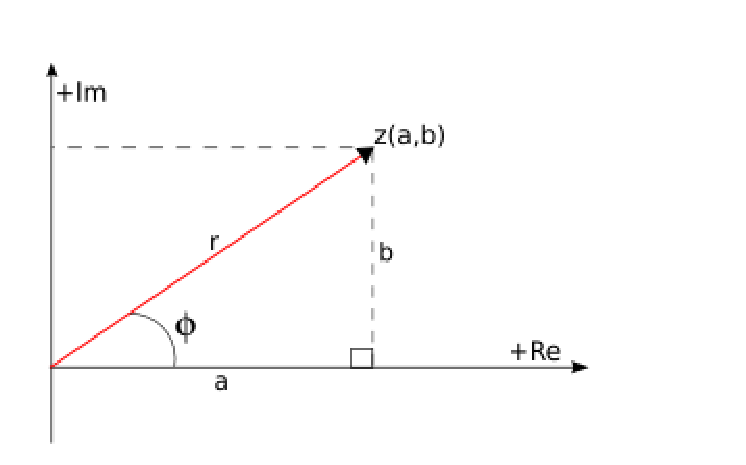
\includegraphics[height=4cm,width=6cm]{complejo1.eps}
\end{minipage}
\hfill
\\

Si $\theta = Arg(z)$:

\quad$tg(\theta)=\dfrac{a}{b}$

Por tanto: Si $a=0$ \quad $(z=bi)$

\qquad\qquad • Si $b=0$, $z=0$ No tiene argumento. El complejo se ubica en el origen de cordenadas.\\

\qquad\qquad • Si $b>0$, $Arg(z)=\dfrac{\pi}{2}$ El complejo se ubica en la parte positiva del eje de las ordenadas.\\

\qquad\qquad • Si $b<0$, $Arg(z)=\dfrac{3}{2}\pi$ El complejo se ubica en la parte negativa del eje de las ordenadas.

\paragraph{Forma Trigonometrica}
\section{Forma Trigonometrica}

Sea $z=a+bi \in \mathbb{C}$, $\theta=Arg(z)$ y $r=|z|$. 

Sabiendo:

\quad • $sen(\theta)=\dfrac{b}{r} \Rightarrow b=r\times sen(\theta)$

\quad • $cos(\theta)=\dfrac{a}{r} \Rightarrow a=r\times cos(\theta)$
				
Definimos la forma Trigonometrica como la siguiente:
$$z= r\times(sen(\theta)+i \times cos(\theta))$$


Ejemplo:
----

\subsection{Propiedades de modulo y argumento}

Sean $z,w \in \mathbb{C}$:

\quad • $|zw|=|z|\times|w|$

\quad • $Arg(z)+Arg(w)$ es un $Arg(zw)$


Demostracion:

\quad Sea $|z|=P$, $Arg(z)=\theta$ \quad $|w|=J$, $Arg(w)=\alpha$:

$$zw=[P\times (sen(\theta)+i \times cons(\theta))]\times [J(sen(\alpha)+i\times cos(\alpha))]=$$
$$=P\times J [cos(\theta)\times cos(\alpha)+i\times cos(\theta)\times sen(\alpha)+i\times sen(\theta)\times cos(\alpha)-sen(\theta)\times sen(\alpha)]=$$
$$=P \times L [\underbrace{(cos(\theta)\times cos(\alpha)- sen(\theta)\times sen(\alpha))} _{cos(\theta+\alpha)}+ i \times \underbrace{(sen(\theta)\times cos(\alpha)+cos(\theta)\times sen(\alpha))} _{sen(\theta +\alpha)}=$$
$$=P \times L [cos(\theta + \alpha)+ i \times sen(\theta + \alpha)]$$

$\therefore |zw|=P \times L=|z| \times |w|$\\

Un argumento de $zw$ es $Arg(z)+Arg(w)$\\

\paragraph{Corolario: Propiedades}
\quad \\

$zw=(PL)_{\theta +\alpha}$\\

$\dfrac{z}{w} = \left( \dfrac{P}{L} \right) _{\theta + \alpha}$ $\forall w \neq 0$\\

$z^n=(P^n)_{n\theta}$\\
\\
Demostracio:

$\dfrac{z}{w}=zw^{(-1)}$

Sabemos: $w\times w^{(-1)}$

Luego $|w\times w^{(-1)}|=1 \Rightarrow |w^{(-1)}|=\dfrac{1}{|w|}$

Notaremos como $arg(z)$ a algun argumento, no al principal, de z.

$\left. \begin{array}{c}
Arg(1)=0 \\
arg(w\times w ^{(-1)})=arg(w)+arg(w^{(-1
)}\\
\end{array} \right\} \Rightarrow arg(w)+arg(w^{(-1)})=0 \Rightarrow arg(w^{(-1)}) = -arg(w)$

$\therefore \dfrac{z}{w}=zw^{(-1)}=\left(PL\right)_(\theta - \alpha)$\\
\\
Ejemplo:
-----

\subsection{Igualdad en Forma Polar}

Sean $z=L_\theta$, $w=P_\alpha$

$$z=w \Leftrightarrow \left\{ \begin{array}{c c c}
L=& P &\\
\theta = & \alpha + k \times 2\pi & \forall k \in \mathbb{Z} \\
\end{array} \right.$$

\section{Raices n-esimas de una complejo}

Definicion: dado $w \in \mathbb{C}$, y $n \in \mathbb{N}$ decimos que $z \in \mathbb{C}$ es raiz n-esima de $w$ si $z^n=w$

Ejemplo: Calcular la raiz cuarta de $w=16_{\dfrac{\pi}{4}}$

\quad Sea $z=P_\theta$ una raiz cuarta de $w$. Entonces $z^4=w$ y como $z^4=(P^4)_{4\theta}$ 

\quad $\therefore \left\{ \begin{array}{c c c}
P^4 = & 16 & \\
4\theta = & \dfrac{\pi}{4} +2k\pi & \forall k \in \mathbb{Z}\\
\end{array}\right.$


\qquad • $P^4 =16 \Rightarrow P=2$

\qquad • $\theta = \dfrac{\dfrac{\pi}{4} +2k\pi}{4}= \dfrac{\pi}{16}+\dfrac{2k\pi}{4}$ \quad $\forall k \in \mathbb{Z}$


Procedemos dando valores a $k$.

(k=0) $\theta _0 =\dfrac{\pi}{16}$ \quad (k=1) $\theta _1 = \dfrac{9}{16} \pi$

(k=2) $\theta _2=\dfrac{17}{16} \pi$ \quad (k=3) $\theta _3=\dfrac{25}{16} \pi$

Notamos que si pasamos el n-esimo valor para $k$ en este caso el 4, repetiremos resultados por lo tanto el procedimiento termina ahi. Esas son las 4 raices cuartas de nuestro $z$.

\paragraph{Teorema de Movie} Lo mostrado anteriormente se resumen con este teorema de la siguiente manera.

Dado $w=P_\theta \in \mathbb{C}$ y $n \in \mathbb{N}$ entonces $w$ tiene $n$ raices n-esimas. $z=L_\alpha \in \mathbb{C}$ donde:

$$\left\{ \begin{array}{c c c}
L= & \sqrt[n]{P} &\\
\alpha = & \dfrac{\theta+2k\pi}{n} \quad \forall k \in {0,1,...,n-1} \\

\end{array} \right.$$






%\input{cap2.Polinomios.tex}
%\input{cap3.Conjuntos.tex}
%\input{cap4.Relaciones.tex}
%\input{cap5.Funciones.tex}
%\input{cap6.Vectores.tex}
%\input{cap7.ReactayPlano.tex}
%\input{cap8.InecuacionesLineales.tex}


\end{document}
